\chapter{Predictive Formulation and System Design}\label{ch:4}

This chapter develops the predictive system. Section 4.1 formalises the task and fixes notation. Section 4.2 presents the obvious formulation, the independent multi-horizon classifier, and shows why it is structurally defective. Section 4.3 presents the discrete-time survival formulation adopted in its place, and Section 4.4 gives its likelihood under censoring. Section 4.5 explains why class reweighting, the standard reflex on a rare-event task, is inadmissible under this formulation. Sections 4.6 and 4.7 describe the features and the models. Section 4.8 describes calibration, Section 4.9 the evaluation protocol, Section 4.10 the risk-control procedure, and Section 4.11 the point-process analysis used to characterise handover clustering.

Each modelling subsection is presented in the same order: the problem that motivates the component, the design of the component, and the technical advantage it confers over the alternative it replaces.


\section{Problem formalisation}
\label{sec:4_1}

Let a drive d consist of samples indexed by t on a uniform one-second grid. At each sample the handset observes a feature vector xt constructed from measurements available at or before t. Let Tt denote the time remaining from t until the next handover command on the same drive.

The task is to estimate, for a set of horizons $h_1 < h_2 < \dots < h_K$, the cumulative incidence


\begin{equation}\label{eq:4_1} F_k(x_t) = P( T_t \le h_k \mid x_t ), \quad k = 1, \dots, K \end{equation}

with K = 5 and horizons of 0.5, 1, 2, 3 and 5 seconds. Samples for which the drive ends before the next handover occurs are right-censored: the event is known not to have occurred within the observed window, but its eventual time is unknown. The formulation that follows handles such samples, and Section 4.4 gives the likelihood that does so. It should be said immediately, however, that on this dataset the machinery is exercised by nothing: the row filter of Section 4.1 keeps only rows carrying a full five-second follow-up window inside their own campaign, so no retained row is censored inside the horizon grid. The censoring treatment is therefore developed because the formulation is not specific to these four campaigns --- a longer horizon grid or a shorter session would make it bind --- and it is not counted anywhere in this thesis as an advantage the measurements demonstrate.


\begin{table}[htbp]
\centering
\caption{Positive-class prevalence by horizon on the common row set, and the accuracy obtained by a constant negative prediction.}
\label{tab:4_1}
\vspace{0.4em}
\singlespacing
\small
\begin{tabularx}{\linewidth}{X c c}
\toprule
\textbf{Horizon} & \textbf{Prevalence} & \textbf{Accuracy of a constant ``no handover''} \\
\midrule
0.5 s & 3.7 \% & 96.3 \% \\
1 s & 6.8 \% & 93.2 \% \\
2 s & 12.6 \% & 87.4 \% \\
3 s & 17.6 \% & 82.4 \% \\
5 s & 26.1 \% & 73.9 \% \\
\bottomrule
\end{tabularx}
\end{table}


\section{The multi-horizon binary formulation and its defect}
\label{sec:4_2}

Motivation. The most direct approach to Equation (4.1) is to define, for each horizon, a binary label yt,k = 1{ Tt $\le$ hk } and fit K independent classifiers. This is the formulation implied by every model in the audit of Section 2.3 that predicts at more than one horizon, and it requires no special machinery.

The defect. The K classifiers are fitted independently and are therefore free to produce estimates that violate the ordering implied by their own definitions. Because the event { T\_t $\le$ h1 } is contained in { T\_t $\le$ h2 } whenever h1 < h2, the probabilities must satisfy F1 $\le$ F2 $\le$ \dots{} $\le$ FK at every sample. Independent fits do not enforce this, and Section 5.4 measures how often they violate it: on 40.2\% of rows.

A violation is not a small numerical irregularity. It is an assertion that a handover is more likely within one second than within three, which is impossible, and it destroys the interpretation of the output as a probability. An operator presented with such a pair of numbers cannot act on either.

Why post-hoc repair is not free, and where it is. The defect can be repaired after the fact by projecting the K outputs onto the monotone cone --- a per-row cumulative maximum, or the pool-adjacent-violators projection --- or by calibrating each horizon separately with the isotonic regression of Zadrozny and Elkan \cite{ref34}, which is the standard non-parametric alternative to the temperature scaling of Guo et al. \cite{ref33} and is preferred here because unconstrained temperature scaling fitted separately per horizon does not preserve cross-horizon ordering, whereas isotonic calibration non-parametrically aligns probability-frequency agreement directly. All three repairs are implemented and reported in Section 5.4 as controls, and the first two need no held-out split and reach zero violations by construction, exactly as the hazard formulation does. What remains of the case for the hazard formulation, after the concessions this section and Section 5.4 make, is narrow and should be stated as such: it achieves coherence from one fit rather than five, and it calibrates better than the projected controls at the horizons where the output is usable as a probability. Two advantages claimed for it elsewhere in the literature do not apply to this data and are withdrawn here. It does not rank better --- Section 5.4 measures the hazard arm slightly below the independent control, well inside the per-campaign spread. And it does not inherit any benefit from the censoring treatment of Section 4.4, because no row in this dataset is censored inside the horizon grid; the censoring-aware likelihood is correct and general, and on these four campaigns it is inert. That leaves a convenience argument and a calibration argument, and the abstract and Chapter 7 now say so.


\section{The discrete-time survival formulation}
\label{sec:4_3}

Motivation. The ordering constraint is a consequence of the definition of cumulative incidence, so the natural remedy is to estimate a quantity from which ordering follows automatically, rather than to estimate the ordered quantities directly and repair them. The discrete-time survival formulation itself has deep foundations in event-history analysis (Prentice and Gloeckler \cite{ref48}, Allison \cite{ref49}, and Tutz and Schmid \cite{ref50}).

Design. Partition the time axis into K bins whose upper edges are exactly the horizons of interest:

B\_1 = (0, h\_1],  B\_2 = (h\_1, h\_2],  \dots{},  B\_K = (h\_{K$-$1}, h\_K]

and define the discrete-time hazard as the probability that the event falls in bin k given that it has not occurred by the start of that bin:


\begin{equation}\label{eq:4_2} \lambda_k(x) = P( T \in B_k \mid T > h_{k-1}, x ) \end{equation}

The survival function is the product of per-bin survivals,


\begin{equation}\label{eq:4_3} S_k(x) = \prod_{j=1}^k ( 1 - \lambda_j(x) ) = P( T > h_k \mid x ) \end{equation}

and the cumulative incidence required by Equation (4.1) is its complement, which is the product-limit identity:


\begin{equation}\label{eq:4_4} F_k(x) = P( T \le h_k \mid x ) = 1 - \prod_{j=1}^k ( 1 - \lambda_j(x) ) \end{equation}

Technical advantage. Monotonicity is now a theorem rather than a hope. Since $\lambda$j $\in$ [0,1], every factor (1 $-$ $\lambda$j) lies in [0,1], so


\begin{equation}\label{eq:4_5} S_{k+1} = S_k \cdot ( 1 - \lambda_{k+1} ) \le S_k \implies F_{k+1} \ge F_k \end{equation}

The argument uses no property of the learner beyond the range of its output. Any model that emits a value in [0,1] per bin produces a coherent set of horizon probabilities under Equation (4.4). This is why the coherence result reported in Section 5.4 is learner-independent while the calibration result is not, and it is the single most important structural property of the system developed here.


\begin{figure}[htbp]
\centering
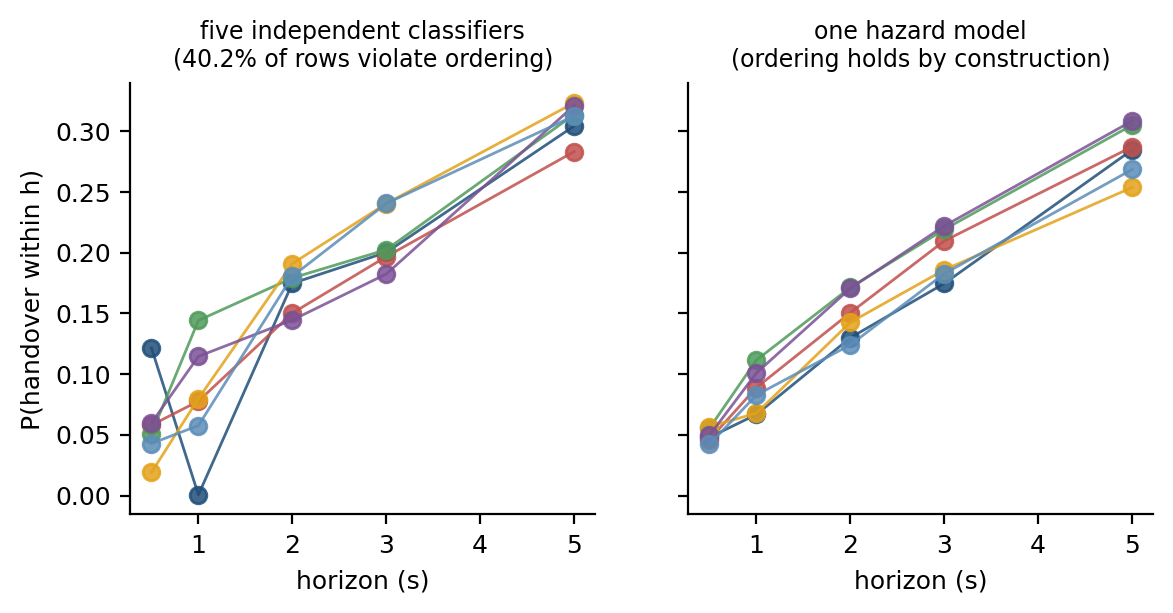
\includegraphics[width=0.85\linewidth]{figures/fig_c11_schematic.png}
\caption{Independent per-horizon classifiers against the hazard formulation, drawn on simulated rows. The hazard formulation enforces monotonicity across horizons by construction.}
\label{fig:4_1}
\end{figure}


\section{The likelihood under censoring}
\label{sec:4_4}

Let kt be the bin in which the event occurs for sample t, and let ct be the last bin fully survived before censoring. Define the at-risk set Rt = {1 \dots{} min(kt, ct)} --- the bins the sample actually entered --- and the per-bin indicator zt,k = 1{ k = kt }. The discrete-time survival log-likelihood then collapses into a single expression covering both the censored and uncensored cases:


\begin{equation}\label{eq:4_6} \ell = \sum_t \sum_{k \in R_t} \left[ z_{t,k} \log \lambda_k(x_t) + (1 - z_{t,k}) \log (1 - \lambda_k(x_t)) \right] \end{equation}

Equation (4.6) is exactly a binary cross-entropy over the expanded set of (sample $\times$ at-risk bin) pairs, a well-established formulation known as pooled discrete hazard regression (Prentice and Gloeckler \cite{ref48}, Allison \cite{ref49}, Tutz and Schmid \cite{ref50}). The practical consequence is that fitting a discrete-time survival model requires no specialised software: the data are expanded from wide to long format, the bin index k is appended as a feature so that the model can learn the shape of the baseline hazard, and a single binary classifier is fitted. A censored sample contributes a (1 $-$ $\lambda_k$) term for every bin it survived rather than being discarded. The methodological contribution here is not the invention of this classical hazard machinery, but its application to cellular telemetry to ensure exact cross-horizon monotonicity by construction without held-out calibration splits or post-hoc corrections.

On this dataset the expansion takes the 8,586 usable rows to 39,435 (sample, bin) pairs. Because every retained row carries a full five-second follow-up window inside its own campaign, no row is censored inside the horizon grid, and the measured per-bin hazards chain exactly to the prevalences of Table~\ref{tab:4_1} by Equation~\eqref{eq:4_4}. Table~\ref{tab:4_2} reports both, side by side, as an arithmetic check on the implementation.


\begin{table}[htbp]
\centering
\caption{Measured discrete-time hazard by bin, and the cumulative incidence it implies, against the prevalence of Table~\ref{tab:4_1}. The two agree exactly by construction.}
\label{tab:4_2}
\vspace{0.4em}
\singlespacing
\footnotesize
\resizebox{\linewidth}{!}{%
\begin{tabular}{l c c c c c c}
\toprule
\textbf{Bin} & \textbf{Interval} & \textbf{At risk} & \textbf{Events} & \textbf{Hazard} & \textbf{F(h) from hazards} & \textbf{Prevalence (Table~\ref{tab:4_1})} \\
\midrule
1 & (0, 0.5] s & 8,586 & 319 & 0.0372 & 0.0372 & 0.0372 \\
2 & (0.5, 1] s & 8,267 & 264 & 0.0319 & 0.0679 & 0.0679 \\
3 & (1, 2] s & 8,003 & 497 & 0.0621 & 0.1258 & 0.1258 \\
4 & (2, 3] s & 7,506 & 433 & 0.0577 & 0.1762 & 0.1762 \\
5 & (3, 5] s & 7,073 & 730 & 0.1032 & 0.2612 & 0.2612 \\
\bottomrule
\end{tabular}%
}
\end{table}


\section{Why class reweighting is inadmissible here}
\label{sec:4_5}

The standard response to a rare-event task is to reweight the positive class, for example through the scale\_pos\_weight parameter of a gradient-boosting implementation. That response must not be used in the hazard arm, for a reason specific to Equation (4.4).

Reweighting the positive class by a factor w transforms the fitted probability monotonically,


\begin{equation}\label{eq:4_7} \tilde{\lambda} = \frac{w \lambda}{w \lambda + (1 - \lambda)} \end{equation}

Retraining with class weighting alters the gradient balance during optimization and distorts the calibrated probability scale. Furthermore, combining rescaled per-bin hazards across horizons does not generally preserve cumulative incidence rankings across samples. Writing the reweighted hazards as $\lambda_k$ $\approx$ w $\lambda_k$ for small $\lambda_k$, the survival function is transformed as


\begin{equation}\label{eq:4_8} \tilde{S}_k = \prod_j (1 - w \lambda_j) \approx (S_k)^w, \quad \text{so} \quad \tilde{F}_k \approx 1 - (1 - F_k)^w \end{equation}

Equation (4.8) replaces a compounding claim made in an earlier draft of this work, which stated that a per-bin multiplicative error $\epsilon$ grows as $(1+\epsilon)^k$ with the horizon. That is not what the product-limit identity does: for small hazards the relative distortion of $F_k$ is bounded by w and is largest at the shortest horizon, while the absolute distortion grows with $F_k$ and is therefore largest at the longest. Retraining under class weights destroys probability calibration without guaranteeing rank preservation once hazards are multiplied across bins; for these reasons, both the hazard arm and the independent-classifier control arm are fitted unweighted, and the fairness of the comparison between them is a secondary benefit.


\section{Feature construction}
\label{sec:4_6}

Design. The feature vector at the prediction instant $t$ has three blocks and 112 columns in total: 89 radio, 17 mobility and 6 history. The serving radio and mobility blocks are built from the one-hertz export; the history block is built from the decoded signalling. Because the diagnostic CSV export lacks periodic neighbour-cell logging (all candidate \texttt{Best\_N} columns are unpopulated in the raw vendor CSV), candidate neighbour RSRP measurements are causally reconstructed by projecting event-triggered RRC \texttt{MeasurementReport} messages onto the integer-second grid using a backward-looking zero-order hold with a 3.0~s expiration tolerance window. Observation staleness is tracked during ingestion via report age features (\texttt{mr\_age\_s} and \texttt{nbr\_age\_s}) for quality control and logging audits, while the model input vector incorporates six explicit missingness indicator masks. A further 10 signalling and configuration columns are built but withheld from every learner outside the ablation of Section~\ref{sec:5_8}, so the design matrix on disk has 122 columns while the main feature set has 112; Table~\ref{tab:4_3} gives the reconciliation, and every count quoted anywhere in this thesis is generated from it. Two rules govern the construction of the blocks, and the first is the single most consequential decision in this thesis.

Alignment. An export row stamped t summarises an interval that ends after t, not before it: Section~\ref{sec:5_1} shows that in 76\% of handovers the row stamped inside the second before the handover command already carries the post-handover serving cell, against a background rate of 12\% three rows earlier. Every export-derived feature is therefore lagged by one row, so that a prediction made at t uses only the row closing at or before t. Nothing else in this thesis changes as much as this does.

History from the event clock, not from the export. Time since the previous handover command, the number of commands in the previous 30 and 60 seconds, and whether the previous command was a return are computed from the decoded signalling, whose timestamps are recorded with millisecond resolution in the diagnostic log, and over the whole continuous session rather than within a 180-second block. Computing them per block left a third of every block with a truncated history, and computing dwell time from the export's serving-cell column imports the alignment error described above: that single substitution moves the dwell feature's own AUROC from 0.873 to 0.664.

Every rolling window is strictly backward-looking and closes at the lagged row, and window computation is performed per campaign so that no window spans a session boundary. Scalers, imputation values, thresholds and calibrators are fitted inside the training partition of each fold only.


\begin{table}[htbp]
\centering
\caption{Feature blocks, their source and their alignment.}
\label{tab:4_3}
\vspace{0.4em}
\singlespacing
\small
\begin{tabularx}{\linewidth}{l c p{3.8cm} X}
\toprule
\textbf{Block} & \textbf{Count} & \textbf{Source} & \textbf{Content} \\
\midrule
Radio & 89 & 1 Hz export and report projection, lagged one row & Serving RF (RSRP, RSRQ, SINR, RSSI, CQI) and report-projected neighbour RSRP; rolling mean, standard deviation, range, slope and first difference over 3, 5 and 10 s; serving-to-neighbour gaps; missingness indicator masks \\
Mobility & 17 & 1 Hz export, lagged one row & GPS speed, heading change, acceleration, stop duration and mobility state, with their rolling statistics \\
History & 6 & decoded signalling, session-level & Time since the previous and second-previous handover command, command counts in the previous 30 and 60 s, whether the previous command was a return \\
Main feature set & 112 &  & used by every learner in Sections~\ref{sec:5_2} to~\ref{sec:5_8} \\
Signalling (ablation only) & 10 & decoded signalling & A3 and all-event report counts in (t$-$w, t], time since the last A3 report, A3 hold time, and the offset, hysteresis and time-to-trigger in force \\
Design matrix as built & 122 &  & the main set plus the signalling block; learners outside Section~\ref{sec:5_8} are given the main set only \\
\bottomrule
\end{tabularx}
\end{table}

The signalling block is reported as an ablation rather than used in the main arm. It counts measurement reports by event type in the windows (t $-$ w, t] for w in {1, 2, 5} seconds, the time since the most recent A3 report, how long the A3 entry condition has held, and the offset, hysteresis and time-to-trigger in force. These are quantities the network itself holds at t, so using them is legitimate; they are separated out because a handset-side predictor may not have them, and because their contribution is worth reporting on its own (Section~\ref{sec:5_8}).

The signalling block requires an explicit leakage guard. A measurement report is a causal antecedent of the handover it triggers, and it is also, in the log, nearly simultaneous with it. A naive "time since last A3 report" feature therefore carries information about the very handover being predicted. The guard applied here excludes any report falling inside the prediction window itself, so that a signalling feature evaluated at t for horizon h may only reference reports transmitted at or before t. Section~\ref{sec:5_11} reports what happens when the guard is removed.


\section{Models compared}
\label{sec:4_7}

Seven learners are compared under identical folds, identical seeds, the identical hazard formulation and the identical feature matrix. The last of those is a change from an earlier draft, in which the sequence models consumed raw per-second measurements while the tabular models received the engineered features and the history block; under that arrangement the comparison varied the inputs as well as the learner. Here the sequence models consume windows of the ten most recent feature vectors --- the same vectors, lagged the same way --- so the only thing that varies between arms is the learner.

The implemented A3 signal-margin proxy. The A3 entry condition is scored as an empirical predictor using the recovered deployed parameters of Table~\ref{tab:3_1}, determining when the signal margin condition of Equation~\eqref{eq:2_1} holds on the sampled grid. This represents an implemented proxy rather than the complete operator handover controller, since 1~Hz exported telemetry cannot reconstruct the continuous internal eNodeB time-to-trigger timer state. Specifically, the network's deployed TTT values (160--320~ms) are strictly sub-grid relative to the 1~Hz sample interval (1000~ms). On a 1~Hz discrete grid, requiring persistence across $\ge 2$ consecutive sample rows would enforce an elapsed duration of $\ge 2000\text{ ms}$---between 6 and 12 times longer than the true network TTT---which would introduce severe artificial lag rather than emulating the timer. Conversely, evaluating persistence over $\ge 1$ sample on a 1~Hz grid is mathematically identical to checking whether the entry condition holds at that sample. The instantaneous margin proxy is therefore the only physically consistent representation available at 1~Hz, while acknowledging that continuous sub-second eNodeB timer states cannot be emulated on a 1~Hz discrete grid.

Logistic regression. A regularised linear model over the 112 features, included as the simplest learner that can use the full feature set. It is worth noting ahead of Table~\ref{tab:5_5} that this arm is slightly ahead of untuned gradient boosting under the fixed-hyper-parameter ladder. That is a property of the default settings rather than of the model families: a linear decision boundary has little capacity to fit the campaign it was trained on, so it loses least when the test campaign is a different corridor. Under the tuning budget of Table~\ref{tab:5_4} the ordering reverses, which is itself the point of Section~\ref{sec:5_3} -- the protocol reorders the leaderboard, so a leaderboard is not a property of the learners alone.

Gradient-boosted trees. LightGBM \cite{ref32} is adopted as the primary model throughout this thesis. This choice is guided by three architectural properties of gradient-boosted decision trees on mobile telemetry: (i) native handling of missing values, which is critical because candidate neighbour-cell measurements from RRC reports arrive intermittently; (ii) scale invariance to heterogeneous feature types (combining RF power in dBm, SINR in dB, GPS velocity in km/h, heading derivatives in degrees, and discrete event counts); and (iii) high computational throughput, which makes rigorous nested cross-validation and hyperparameter search feasible without downsampling.

Multi-layer perceptron. A feed-forward network over the same tabular features, included to separate the contribution of non-linearity from that of temporal memory.

Sequence models. A temporal convolutional network, a Transformer encoder and a gated recurrent unit, each consuming a window of the ten most recent lagged feature vectors rather than a single instantaneous vector. These arms test whether a model with explicit sequence memory over time windows outperforms gradient-boosted trees receiving hand-constructed rolling statistics.

Every arm receives the same tuning budget: twenty random-search trials per outer fold, sampled from the defined search distributions in Table~\ref{tab:4_4}. To prevent test-set leakage, tuning is strictly nested: inside each outer fold (where one full campaign is held out for testing and three are available for training), the training partition is split chronologically into a 75\% sub-training set and a 25\% internal validation block, separated by a 60-second temporal purge to suppress boundary autocorrelation. Hyperparameter configurations are scored against this internal validation block; the best configuration is then refitted on the combined training partition before scoring the outer held-out campaign.


\begin{table}[htbp]
\centering
\caption{Hyperparameter search spaces for the evaluated learners. Each outer fold draws 20 random configurations evaluated on a purged 25\% internal validation partition.}
\label{tab:4_4}
\vspace{0.4em}
\singlespacing
\small
\begin{tabularx}{\linewidth}{l p{4.2cm} X}
\toprule
\textbf{Learner} & \textbf{Hyperparameter} & \textbf{Search range and distribution} \\
\midrule
\multirow{6}{*}{LightGBM} 
  & \texttt{learning\_rate} & Log-uniform $[0.01, 0.2]$ \\
  & \texttt{num\_leaves} & Integer uniform $[7, 63]$ \\
  & \texttt{min\_data\_in\_leaf} & Integer uniform $[10, 200]$ \\
  & \texttt{feature\_fraction} & Uniform $[0.4, 1.0]$ \\
  & \texttt{lambda\_l2} & Log-uniform $[10^{-3}, 10.0]$ \\
  & \texttt{n\_estimators} & Integer uniform $[100, 800]$ \\
\midrule
Logistic Regression 
  & Inverse regularization $C$ & Log-uniform $[10^{-3}, 10.0]$ (L2, L-BFGS, max\_iter=3000) \\
\midrule
\multirow{3}{*}{MLP} 
  & Hidden units (2 layers) & Categorical $\{32, 64, 128, 256\}$ \\
  & L2 penalty $\alpha$ & Log-uniform $[10^{-5}, 10^{-1}]$ \\
  & Initial learning rate & Log-uniform $[10^{-4}, 10^{-2}]$ (AdamW, early stopping) \\
\midrule
\multirow{4}{*}{\shortstack[l]{Sequence models\\(GRU, TCN, Trans.)}} 
  & Hidden dimension & Categorical $\{16, 32, 64\}$ (lookback window $W=10$) \\
  & Learning rate & Log-uniform $[3 \times 10^{-4}, 3 \times 10^{-3}]$ \\
  & Dropout & Uniform $[0.0, 0.4]$ \\
  & Weight decay & Log-uniform $[10^{-6}, 10^{-3}]$ (AdamW, 25 epochs) \\
\bottomrule
\end{tabularx}
\end{table}

What that nesting does and does not protect against should be stated, because the totals involved are large: twenty trials across seven learners, four protocols, four outer folds and three seeds, on a row set carrying roughly six hundred positive rows at the one-second horizon. What it protects against is selection on the test campaign: no held-out campaign is ever scored during a search, so the reported metric for any one arm is not an optimised quantity. What it does not remove is selection across arms. The best of seven learners is reported beside the other six, and when the best and the second-best differ by less than the width of their own bootstrap intervals --- which Section 5.2 shows is the usual case --- the ranking between them is not a finding, and this thesis does not treat it as one. 

Multiplicity and hypothesis testing scope. For model family comparisons across the leaderboard, no multiplicity correction is applied: because differences between top-ranking learners fall well within the width of their block-bootstrap intervals, these comparisons are treated descriptively rather than as formal null-hypothesis rejections, and the reader is given the full table and the intervals instead. Conversely, for formal statistical goodness-of-fit hypothesis testing --- specifically the Kolmogorov--Smirnov residual tests evaluating the self-exciting Hawkes process across campaigns in Section~\ref{sec:5_10} --- multiplicity control is strictly enforced via the Holm--Bonferroni procedure across the four campaigns. Every comparative claim in Chapter 5 is stated as a paired difference with an interval rather than as an ungrounded ordering of point estimates.


\section{Calibration}
\label{sec:4_8}

Ranking quality is insufficient for the task stated in Section 1.3, which requires the asserted probability to correspond to an empirical frequency. Three calibration treatments are evaluated.

Temperature scaling \cite{ref33} fits a single scalar on a held-out partition, dividing the logits before the sigmoid. It is the least expressive treatment and cannot alter the ranking.

Isotonic regression \cite{ref34} fits a non-decreasing step function per horizon. It is more expressive and can correct a wider class of miscalibration, but it consumes a held-out split and, applied per horizon, is free to reorder the horizons relative to one another.

The monotone projection repairs an incoherent set of horizon outputs by projecting them onto the monotone cone. It is implemented for the control arm only, since the hazard formulation makes it unnecessary.

Calibration quality is reported as the expected calibration error, computed as the weighted mean absolute difference between confidence and empirical frequency across equal-mass bins, with the Brier score reported alongside it.


\section{Evaluation protocol}
\label{sec:4_9}

Motivation. The protocol is the component most likely to invalidate a result on data of this kind, for two reasons that are usually conflated. Adjacent one-second samples within a session are near-duplicates, so a random row split places nearly the same row on both sides of it. But 180-second blocks of one continuous session are not independent either: they share cells, traffic, weather, device state and driver. Section 5.3 measures both.

Design. The evaluation protocol has five elements, and a ladder of four splitting rules is reported rather than one.

Splitting ladder. Four splitting rules are compared: leave-one-campaign-out, which holds out a whole continuous session; blocked cross-validation with a 60-second purge following Roberts et al. \cite{ref35}; random 180-second blocks of one campaign, which is the protocol this work used before the audit; and random rows, which is the protocol most of the comparator literature uses. Section 5.3 reports all four.


\begin{figure}[htbp]
\centering
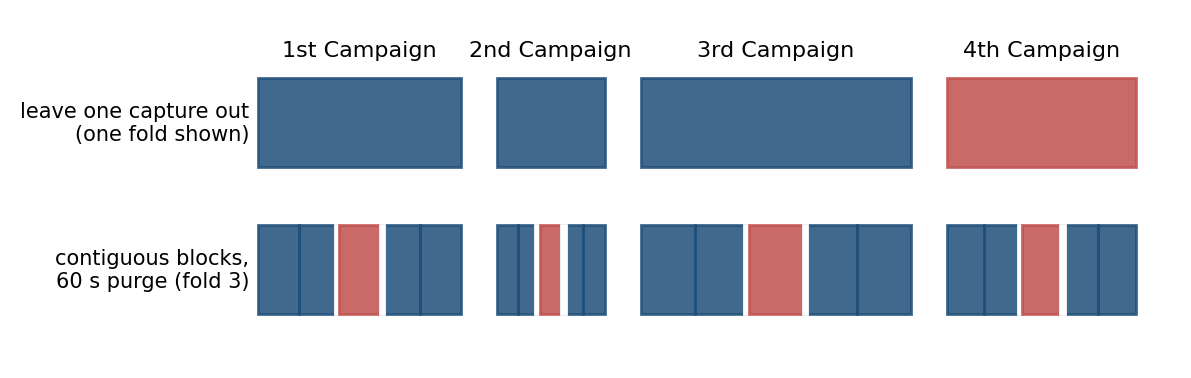
\includegraphics[width=0.85\linewidth]{figures/fig_c1_protocols.png}
\caption{The splitting ladder. Leave-one-campaign-out holds out a whole continuous session; blocked splitting holds out time blocks; random-row splitting holds out individual samples, allowing near-duplicate rows across splits.}
\label{fig:4_2}
\end{figure}

Repetition and uncertainty. Stochastic learners are run over three seeds and their predictions averaged. Intervals on pooled out-of-fold metrics come from a bootstrap that resamples whole 180-second blocks within each campaign; that interval is conditional on these four sessions and does not include between-day variation, so the per-campaign spread is always reported beside it. Comparisons between learners are reported as per-campaign differences over four paired observations, with the exact sign-test p-value quoted only to show its own resolution limit (0.125 at best). No significance claim is made from four units.

Fold hygiene. The feature scaler, the decision threshold, the probability calibrator and the conformal threshold are fitted inside the training or calibration partition of each fold only, and the calibration partition is separated from the training partition by the same 60-second purge.

Metrics. Four families are reported. Ranking quality is reported as AUPRC, always with the prevalence floor and the lift over it, together with AUROC. Calibration is reported as expected calibration error over fifteen equal-mass bins and Brier score. Coherence is reported as the fraction of rows on which the horizon ordering is violated, with the magnitude of the violations. Event-level cost is reported as the fraction of handover commands detected, the number of false-alarm episodes per hour and per kilometre, and the distribution of lead times. Reporting all four families is deliberate: Wagner et al. \cite{ref30} show that no single aggregate metric for event detection satisfies all desirable properties.


\section{Distribution-free risk control}
\label{sec:4_10}

Motivation. A probability is not yet an operating point. An operator needs a decision rule: issue an alarm when the predicted probability exceeds a threshold. A conventional threshold minimizes a cost or targets a point on a receiver operating characteristic, but offers no guarantee on future performance. Conformal risk control \cite{ref21}, which extends the risk-controlling prediction sets of Bates et al. \cite{ref22} from a coverage guarantee to a guarantee on any bounded monotone loss, certifies that the expected risk on unseen test units does not exceed a chosen level $\alpha$.

The exchangeable unit and the loss. The risk is defined per driving unit, not per sample. For a unit d and decision threshold $\lambda$ $\in$ [0, 1]---where an alarm is issued whenever p\_t $\ge$ $\lambda$---the row-level miss loss is the fraction of that unit's positive rows falling below the alarm threshold,


\begin{equation}\label{eq:4_9} R_d(\lambda) = \frac{|\{ t \in d : y_t = 1 \text{ and } \hat{p}_t < \lambda \}|}{\max(|\{ t \in d : y_t = 1 \}|, 1)} \end{equation}

which is bounded in [0, 1] with B = 1. As the decision threshold $\lambda$ increases, the alarm rule becomes stricter, alarms become rarer, and the miss loss R\_d($\lambda$) is non-decreasing in $\lambda$. Under Theorem 1 of Angelopoulos et al. \cite{ref21}, expected risk control E[R\_{n+1}($\lambda$)] $\le$ $\alpha$ is achieved by selecting the most conservative (largest) threshold whose finite-sample empirical bound satisfies the target:


\begin{equation}\label{eq:4_10} \hat{\lambda} = \sup \left\{ \lambda \in [0, 1] : \frac{n \hat{R}(\lambda) + B}{n + 1} \le \alpha \right\} \end{equation}

with $\lambda$ = 0 as the fallback if no threshold satisfies the inequality (which achieves zero miss loss by alarming continuously, bounded by B = 1). This is a statement about rows, and it is not the statement Section 1.3 promises. A network operator misses a *handover*, not a row, and a handover occupies several rows of its lead window. The event-level loss is therefore also carried through: writing E\_d for the handover commands whose lead window lies in unit d, a command at $\tau$ is caught at horizon h if some usable row in [$\tau$ $-$ h, $\tau$) alarms, and


\begin{equation}\label{eq:4_11} R_d^{\text{ev}}(\lambda) = \frac{|\{ \tau \in E_d : \max_{t \in [\tau-h, \tau)} \hat{p}_t < \lambda \}|}{|E_d|} \end{equation}

A command with no usable row in its window is counted as missed rather than dropped from the denominator, which is what makes this loss comparable with the detection rate of Appendix A rather than with the row-level miss rate. Section 5.5 reports both, because they differ and because the difference is the interesting part.

$\hat{R}(\lambda)$ averages the chosen loss over calibration units. The choice of unit is the substantive part of the claim, and it is tested rather than asserted. Section~\ref{sec:5_5} reports the procedure twice: once in an exchangeable reference regime over the pooled 57 blocks, and once across campaigns. 

Crucially, the observations across the 57 blocks are populated from \emph{out-of-fold predictions} generated by the four leave-one-campaign-out models: for each campaign $c \in \{1, 2, 3, 4\}$, the predictor was fitted and tuned on the remaining three campaigns, producing predictions on campaign $c$ that are strictly out-of-fold. In the exchangeable pooled experiment, the 57 blocks carrying these out-of-fold predictions are repeatedly split into calibration ($n \approx 43$) and test units ($n \approx 14$) via a 75/25 partition. Because every prediction was generated by an estimator that never observed that campaign during fitting or hyperparameter tuning, the calibration-test split over out-of-fold predictions evaluates threshold calibration without data leakage. In contrast, cross-campaign deployment evaluates across distinct physical corridors where exchangeability fails under distribution shift.


\begin{equation}\label{eq:4_12} \alpha \ge \frac{1}{n+1} \iff n \ge \frac{1}{\alpha} - 1 \end{equation}

Equation~\eqref{eq:4_12} gives the finite-sample feasibility condition for the empirical bound of \cite{ref21}: for the term $(n \hat{R}(\lambda) + B)/(n+1)$ to reach $\alpha$ when empirical loss is zero ($\hat{R} = 0$), the target must satisfy $\alpha \ge 1/(n+1)$. This is not an impossibility theorem for risk control itself (since the trivial fallback $\lambda = 0$ guarantees zero loss by alarming on all eligible rows), but rather the sample-size floor required for non-trivial threshold selection: a study wishing to promise a non-trivial 5\,\% miss rate without defaulting to continuous alarm needs at least 19 calibration units, and one promising 2\,\% needs 49. Because the four campaigns contain 15, 8, 20, and 14 blocks (mean $n = 14.25$), the calibration size in cross-campaign rotations is fold-specific ($n \in \{8, 14, 15, 20\}$), yielding feasibility floors from 0.048 to 0.111. Only rotations calibrating on the 20-block campaign can express $\alpha = 0.05$ non-trivially.

A second floor binds the event-level loss under the evaluation protocol, arising from preprocessing and blanking rules rather than from calibration sample size. Under the evaluation policy, a 2~s post-handover blanking window is enforced to suppress post-transition transients. A command that follows another within 2~s has no eligible prediction rows in its 1-second lead window $[\tau - 1, \tau)$ and cannot be alarmed. Alarming on every eligible row ($\lambda = 0$) cannot recover events that possess no eligible rows under this policy; continuous alarm only bypasses that floor if the blanking policy itself is abandoned. Across the corpus, 36.4\,\% of one-second lead windows are in that position (against 35.8\,\% in the unbroken sequence, and 12.0\,\% at three seconds). Because the burst density varies across corridors, fold-specific floors range from $\approx 22\%$ on highway routes to over 40\% in dense urban loops, setting the tightest promise a study can certify on handovers.


\section{Point-process analysis of handover arrivals}
\label{sec:4_11}

Motivation. The ping-pong behaviour of Section 5.10 suggests that handovers do not arrive independently. Quantifying that clustering requires a model of the arrival process itself rather than of the per-sample probability.

Design. The handover arrival stream on each drive is modelled as a self-exciting Hawkes process \cite{ref23}, \cite{ref24} with conditional intensity


\begin{equation}\label{eq:4_13} \mu(t) = \mu_0 + \sum_{t_i < t} \alpha \cdot \exp( -\beta ( t - t_i ) ) \end{equation}

in which each arrival raises the intensity of subsequent arrivals by $\alpha$ and the excitation decays at rate $\beta$. The branching ratio $\alpha$/$\beta$ is the expected number of direct offspring per event under this kernel, and summarises the strength of the clustering. Section 5.10 reports that the Ogata residual test rejects the exponential kernel on this data, so that reading is withdrawn there and the ratio is used only as a comparable summary statistic.

Validation. A fit alone is not evidence of self-excitation. Following the networking precedent of Price-Williams and Heard \cite{ref26}, the fit is validated by the residual analysis of Ogata \cite{ref25}: the time axis is rescaled by the fitted compensator, and the transformed inter-arrival times are tested against a unit-rate exponential distribution by a Kolmogorov--Smirnov test on held-out drives. Section 5.10 reports both the branching ratio and the outcome of that test, including the respect in which the test rejects the fitted kernel.

